% pdflatex first-ten-problems.tex && del first-ten-problems.aux, first-ten-problems.out, first-ten-problems.log && start first-ten-problems.pdf
% cd ..\..\Users\NikitaSkybytskyi\Desktop\c3s1\complex-analysis
\documentclass[a4paper, 12pt]{article}
\usepackage[utf8]{inputenc}
\usepackage[english, ukrainian]{babel}

\usepackage{amsmath, amssymb}
\usepackage{multicol}
\usepackage{graphicx}
\usepackage{float}
\usepackage{multicol}

\usepackage{amsthm}
\newtheorem{theorem}{Теорема}[subsection]
\newtheorem*{theorem*}{Теорема}
\newtheorem{lemma}{Лема}[subsection]
\newtheorem*{lemma*}{Лема}
\newtheorem*{remark*}{Зауваження}
\theoremstyle{definition}
\newtheorem*{definition}{Визначення}
\newtheorem{problem}{Задача}[section]
\newtheorem*{solution}{Розв'язок}
\newtheorem{example}{Приклад}
\newtheorem*{example*}{Приклад}
\newtheorem*{hint}{Вказівка}

\newcommand{\Max}{\displaystyle\max\limits}
\newcommand{\Sum}{\displaystyle\sum\limits}
\newcommand{\Int}{\displaystyle\int\limits}
\newcommand{\Lim}{\displaystyle\lim\limits}

\newcommand{\RR}{\mathbb{R}}
\newcommand{\ZZ}{\mathbb{Z}}

\newcommand*\diff{\mathop{}\!\mathrm{d}}
\newcommand*\Diff[1]{\mathop{}\!\mathrm{d^#1}}

\DeclareMathOperator{\Real}{Re}
\DeclareMathOperator{\Imag}{Im}

\DeclareMathOperator{\Arg}{Arg}

\DeclareMathOperator{\Ln}{Ln}

\DeclareMathOperator{\Arctan}{Arctan}
\DeclareMathOperator{\Arcsin}{Arcsin}
\DeclareMathOperator{\Arccos}{Arccos}
\DeclareMathOperator{\Arccosh}{Arccosh}
\DeclareMathOperator{\Arctanh}{Arctanh}

\DeclareMathOperator{\arcsinh}{arcsinh}
\DeclareMathOperator{\arccosh}{arccosh}
\DeclareMathOperator{\arctanh}{arctanh}
\DeclareMathOperator{\arccoth}{arccoth}

\newcommand{\varLimsup}{\varlimsup\limits}

\makeatletter
\newcommand\xLeftrightarrow[2][]{%
  \ext@arrow 9999{\longLeftrightarrowfill@}{#1}{#2}}
\newcommand\longLeftrightarrowfill@{%
  \arrowfill@\Leftarrow\relbar\Rightarrow}
\makeatother

\renewcommand{\epsilon}{\varepsilon}
\renewcommand{\phi}{\varphi}

\allowdisplaybreaks
\setlength\parindent{0pt}
\numberwithin{equation}{subsection}

\usepackage{xcolor}
\usepackage{hyperref}
\hypersetup{unicode=true,colorlinks=true,linktoc=all,linkcolor=red}

\numberwithin{equation}{section}% reset equation counter for sections
\numberwithin{equation}{subsection}
% Omit `.0` in equation numbers for non-existent subsections.
\renewcommand*{\theequation}{%
  \ifnum\value{subsection}=0 %
    \thesection
  \else
    \thesubsection
  \fi
  .\arabic{equation}%
}


\numberwithin{equation}{section}

\begin{document}

\setcounter{section}{1}

\setcounter{problem}{1}
\begin{problem}
	Знайти модулі і аргументи комплексних чисел ($a$ і $b$ -- дійсні числа):
	\begin{multicols}{4}
		\begin{enumerate}
			\item $\dfrac1i$;
			\item $\dfrac{1-i}{1+i}$:
			\item $\dfrac2{1-3i}$;
			\item $\left(1+i\sqrt{3}\right)^3$.
		\end{enumerate}
	\end{multicols}
\end{problem}
\begin{solution}
	Скористаємося правилами арифметичних дій з модулями та аргументами комплексних чисел, а саме 
	\begin{align}
		\label{eq:1.1}
		\left|\frac{z_1}{z_2}\right|&=\frac{|z_1|}{|z_2|},\\
		\arg\left(\frac{z_1}{z_2}\right)&=\arg(z_1)-\arg(z_2),\\
		\left|z_1\cdot z_2\right|&=|z_1|\cdot|z_2|,\\
		\arg(z_1\cdot z_2)&=\arg(z_1)+\arg(z_2).
	\end{align}
	\begin{enumerate}
		\item \[\left|\dfrac1i\right|=\dfrac{|1|}{|i|}=\dfrac11=1.\]
		\[\arg\left(\dfrac1i\right)=\arg1-\arg i=0-\pi/2=-\pi/2.\]
		\item \[\left|\dfrac{1-i}{1+i}\right|=\dfrac{|1-i|}{|1+i|}=\dfrac{\sqrt{2}}{\sqrt{2}}=1.\]
		\[\arg\left(\dfrac{1-i}{1+i}\right)=\arg(1-i)-\arg(1+i)=-\pi/4-\pi/4=-\pi/2.\]
		\item \[\left|\dfrac2{1-3i}\right|=\dfrac{|2|}{|1-3i|}=\dfrac2{\sqrt{10}}=\sqrt{\frac25}.\]
		\[\arg\left(\dfrac2{1-3i}\right)=\arg(2)-\arg(1-3i)=0-\arctan(-3)=-\arctan(-3).\]
		\item \[\left|\left(1+i\sqrt{3}\right)^3\right| = \left|1+i\sqrt{3}\right|^3=2^3=8.\]
		\[\arg\left(\left(1+i\sqrt{3}\right)^3\right)=3\cdot\arg\left(1+i\sqrt{3}\right)=3\cdot\pi/3=\pi.\]
	\end{enumerate}
\end{solution}

\setcounter{problem}{3}
\begin{problem}
	Знайти всі значення наступних коренів (і побудувати їх):
	\begin{multicols}{3}
		\begin{enumerate}
			\item $\sqrt[3]{1}$;
			\item $\sqrt[3]{i}$;
			\item $\sqrt[4]{-1}$;
			\item $\sqrt[6]{-8}$;
			\item $\sqrt[8]{1}$;
			\item $\sqrt{1-i}$;
			\item $\sqrt{3+4i}$;
			\item $\sqrt[3]{-2+2i}$;
			\item $\sqrt[5]{-4+3i}$.
		\end{enumerate}
	\end{multicols}
\end{problem}
\begin{solution}
	Знайдемо значення вищезгаданих коренів через їхні модулі та аргументи, а саме
	\begin{align}
		\label{eq:1.2}
		\left|\sqrt[n]{z}\right|&=\sqrt[n]{|z|},\\
		n\arg\left(\sqrt[n]{z}\right)=n\phi&=\arg(z).
	\end{align}
	\begin{enumerate}
		\item $\left|\sqrt[3]{1}\right| = \sqrt[3]{|1|} = 1$,
		\[3\phi\equiv\arg(1)\implies3\phi\equiv0\implies\phi=\frac{2k\pi}{3},\quad k=0..2.\]
		\item $\left|\sqrt[3]{i}\right| = \sqrt[3]{|i|} = 1$,
		\[3\phi\equiv\arg(i)\implies3\phi\equiv\pi/2\implies\phi=\frac{\pi}{6}+\frac{2k\pi}{3},\quad k=0..2.\]
		\item $\left|\sqrt[4]{-1}\right| = \sqrt[4]{|-1|} = 1$,
		\[4\phi\equiv\arg(-1)\implies4\phi\equiv\pi\implies\phi=\frac{\pi}{4}+\frac{k\pi}{2},\quad k=0..3.\]
		\item $\left|\sqrt[6]{-8}\right| = \sqrt[6]{|-8|} = \sqrt{2}$,
		\[6\phi\equiv\arg(-8)\implies6\phi\equiv\pi\implies\phi=\frac{\pi}{6}+\frac{k\pi}{3},\quad k=0..5.\]
		\item $\left|\sqrt[8]{1}\right| = \sqrt[8]{|1|} = 1$,
		\[8\phi\equiv\arg(1)\implies8\phi\equiv0\implies\phi=\frac{k\pi}{4},\quad k=0..7.\]
		\item $\left|\sqrt{1-i}\right| = \sqrt{|1-i|} = \sqrt[4]{2}$,
		\[2\phi\equiv\arg(1-i)\implies2\phi\equiv-\pi/4\implies\phi=-\frac{\pi}{8}+k\pi,\quad k=0,1.\]
		\item $\left|\sqrt{3+4i}\right| = \sqrt{|3+4i|} = \sqrt{5}$,
		\begin{multline*}2\phi\equiv\arg(3+4i)\implies2\phi\equiv\arctan(4/3)\implies\\\implies\phi=\arctan(4/3)/2+k\pi,\quad k=0,1.\end{multline*}
		\item $\left|\sqrt[3]{-2+2i}\right| = \sqrt[3]{|-2+2i|} = \sqrt{2}$,
		\[3\phi\equiv\arg(-2+2i)\implies3\phi\equiv3\pi/4\implies\phi=\frac{\pi}{4}+\frac{2k\pi}{3},\quad k=0..2.\]
		\item $\left|\sqrt[5]{-4+3i}\right| = \sqrt[5]{|-4+3i|} = \sqrt[5]{5}$,
		\begin{multline*}5\phi\equiv\arg(-4+3i)\implies5\phi\equiv\arctan(-3/4)\implies\\\implies\phi=\arctan(-3/4)/5+\frac{2k\pi}{5},\quad k=0..4.\end{multline*}
	\end{enumerate}
\end{solution}

\setcounter{problem}{7}
\begin{problem}
	Виходячи з геометричних міркувань, довести нерівності
	\begin{multicols}{2}
		\begin{enumerate}
			\item $\left| \dfrac{z}{|z|} - 1 \right| \le |\arg z|$;
			\item $|z - 1| \le | |z| - 1 | + |z| \cdot |\arg z|$.
		\end{enumerate}
	\end{multicols}
\end{problem}
\begin{solution}
	У кожному з пунктів використовується теорема про ту, яку огинають, і ту, яка огинає.
	\begin{enumerate}
		\item LHS -- довжина хорди одиничного кола, що з'єднує точки 1 і $z/|z|$, а RHS -- довжина дуги цього ж кола, що з'єднує ці ж точки, тому LHS $\le$ RHS.
		\item LHS -- довжина відрізку між точками 1 і $z$, а RHS -- сума довжини відрізку між точками 1 і $|z|$ і довжини дуги кола радіусу $|z|$ між точками $|z|$ і $z$, тому LHS $\le$ RHS.
		\begin{figure}[H]
			\centering
			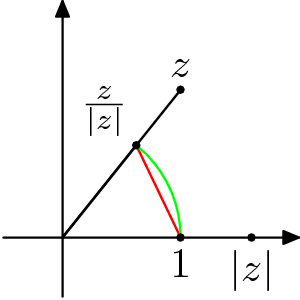
\includegraphics[width=.45\linewidth]{fig-1.png} \qquad
			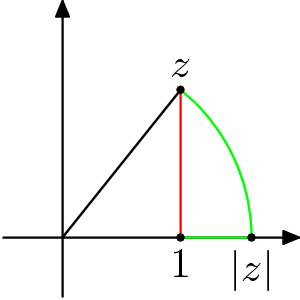
\includegraphics[width=.45\linewidth]{fig-2.png}
		\end{figure}
	\end{enumerate}
\end{solution}

\begin{problem}
	Довести тотожність \[|z_1+z_2|^2+|z_1-z_2|^2=2(|z_1|^2+|z_2|^2),\] і з'ясувати її геометричний зміст.
\end{problem}
\begin{solution}
	Ця тотожність -- ніщо інше як правило паралелограма, ``сума квадратів довжин сторін паралелограма рівна сумі квадратів довжин його діагоналей''.
	\begin{figure}[H]
		\centering
		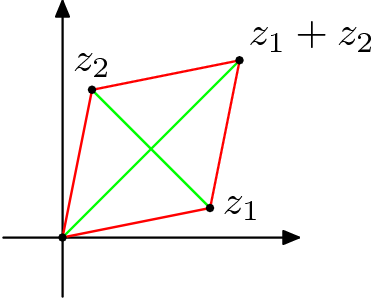
\includegraphics[width=.45\linewidth]{fig-3.png}
	\end{figure}
\end{solution}

\end{document}